\documentclass[tikz]{standalone}
\usepackage{pgfplots}
\pgfplotsset{compat=1.15}
\usepackage{mathrsfs}
\usetikzlibrary{arrows,calc}
\usepackage{tkz-euclide}
\pagestyle{empty}

\definecolor{AngleClr}{rgb}{0,0.39215686274509803,0}
\definecolor{ShapeClr}{rgb}{0.6,0.2,0}
\definecolor{SquareClr}{RGB}{250, 248, 217}
\definecolor{GreenDist}{RGB}{7,122,7}
\definecolor{RedDist}{RGB}{232,57,14}

\begin{document}

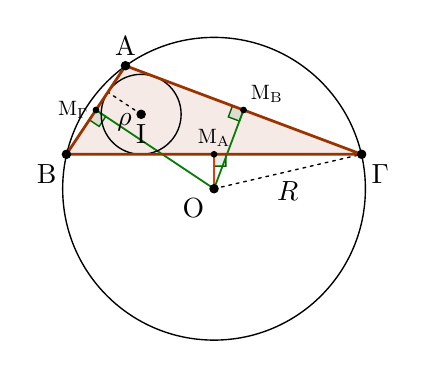
\begin{tikzpicture}[scale=.75]
\tkzSetUpLine[line width=1pt,color=black]
\tkzSetUpPoint[fill=black]

\tkzDefPoints{0/0/B,1/1.5/A,5/0/C}


\tkzDefTriangleCenter[circum](A,B,C) \tkzGetPoint{O}

\tkzDefCircle[in](A,B,C)
\tkzGetPoints{I}{x}


\tkzDefPointBy[projection=onto B--C](O)\tkzGetPoint{OA}
\tkzDefPointBy[projection=onto A--C](O)\tkzGetPoint{OB}
\tkzDefPointBy[projection=onto A--B](O)\tkzGetPoint{OC}

\tkzDefPointBy[projection=onto A--B](I)\tkzGetPoint{IC}


\tkzFillPolygon[fill=ShapeClr,fill opacity=0.1](A,B,C)

\tkzMarkRightAngles[line width=0.5pt, size=.2,color=AngleClr,fill=AngleClr,fill opacity=0.1](O,OC,B O,OA,C O,OB,A)

\tkzDrawSegments[color=GreenDist,line width=0.65pt](O,OA O,OB O,OC)
\tkzDrawSegments[color=RedDist,line width=0.65pt](O,OA)
\tkzDrawSegments[line width=0.5pt,color=black,dashed,dash pattern=on 1pt off 1.75pt](I,IC O,C)

\tkzDrawCircles[line width=0.5pt,color=black](O,A I,x)

\tkzDrawPolygon[color=ShapeClr](A,B,C)

\tkzDrawPoints[size=3](A,B,C,O,I)
\tkzDrawPoints[size=2](OA,OB,OC)

\tkzLabelPoint[above](A){$\rm A$}
\tkzLabelPoint[below left](B){$\rm B$}
\tkzLabelPoint[below right](C){$\rm \Gamma$}
\tkzLabelPoint[below left](O){$\rm O$}
\tkzLabelPoint[scale=0.75,above](OA){$\rm M_A$}
\tkzLabelPoint[scale=0.75,above right](OB){$\rm M_B$}
\tkzLabelPoint[scale=0.75,left](OC){$\rm M_\Gamma$}
\tkzLabelPoint[below](I){$\rm I$}

\tkzLabelSegment[below](I,IC){$\rho$}
\tkzLabelSegment[below](O,C){$R$}

\end{tikzpicture}

\end{document}
